% !TEX root = Projektdokumentation.tex
\section{Anhang}

%\subsection{Detaillierte Zeitplanung}
%\label{app:Zeitplanung}
%\tabelleAnhang{ZeitplanungKomplett}

%\subsection{Gantt-Diagramm}
%\label{app:Gantt}
%\begin{sideways}
%\begin{ganttchart}[
hgrid,
vgrid,
x unit=4mm,
time slot format=isodate
]{2016-04-12}{2016-05-31}
\gantttitlecalendar{year, month, day, week=3, weekday} \\

\ganttbar{}{2016-04-14}{2016-04-17}

\end{ganttchart}

%\end{sideways}


\subsection{API Aufruf: Registrieren eines neuen Benutzers}
\label{app:API_register}
\tabelleAnhang{WebService/register}

\subsection{API Aufruf: Als registrierter Benutzer anmelden}
\label{app:API_login}
\tabelleAnhang{WebService/login}

\subsection{API Aufruf: Einen Raum registrieren}
\label{app:API_register_room}
\tabelleAnhang{WebService/newRoom}

\subsection{API Aufruf: Einen Raum von der Datenbank entfernen}
\label{app:API_delete_room}
\tabelleAnhang{WebService/deleteRoom}

\subsection{API Aufruf: Einen spezifischen Raum abrufen}
\label{app:API_show_room}
\tabelleAnhang{WebService/getRoom}

\subsection{API Aufruf: Eine Liste aller Räume abrufen}
\label{app:API_show_rooms}
\tabelleAnhang{WebService/getRooms}

\subsection{API Aufruf: Ein neues Gerät registrieren}
\label{app:API_register_device}
\tabelleAnhang{WebService/registerDevice}

\subsection{API Aufruf: Ein spezifisches Gerät abrufen}
\label{app:API_get_device}
\tabelleAnhang{WebService/getDevice}

\subsection{API Aufruf: Ein Gerät aus der Datenbank entfernen}
\label{app:API_delete_device}
\tabelleAnhang{WebService/deleteDevice}

\subsection{API Aufruf: Alle Geräte eines Raumes auflisten}
\label{app:API_show_devices}
\tabelleAnhang{WebService/getDevices}

\subsection{API Aufruf: Verändern der Gerätedaten}
\label{app:API_patch_device}
\tabelleAnhang{WebService/patchDevice}




%\subsection{Projektdokumentation Sommersemester 2015}
%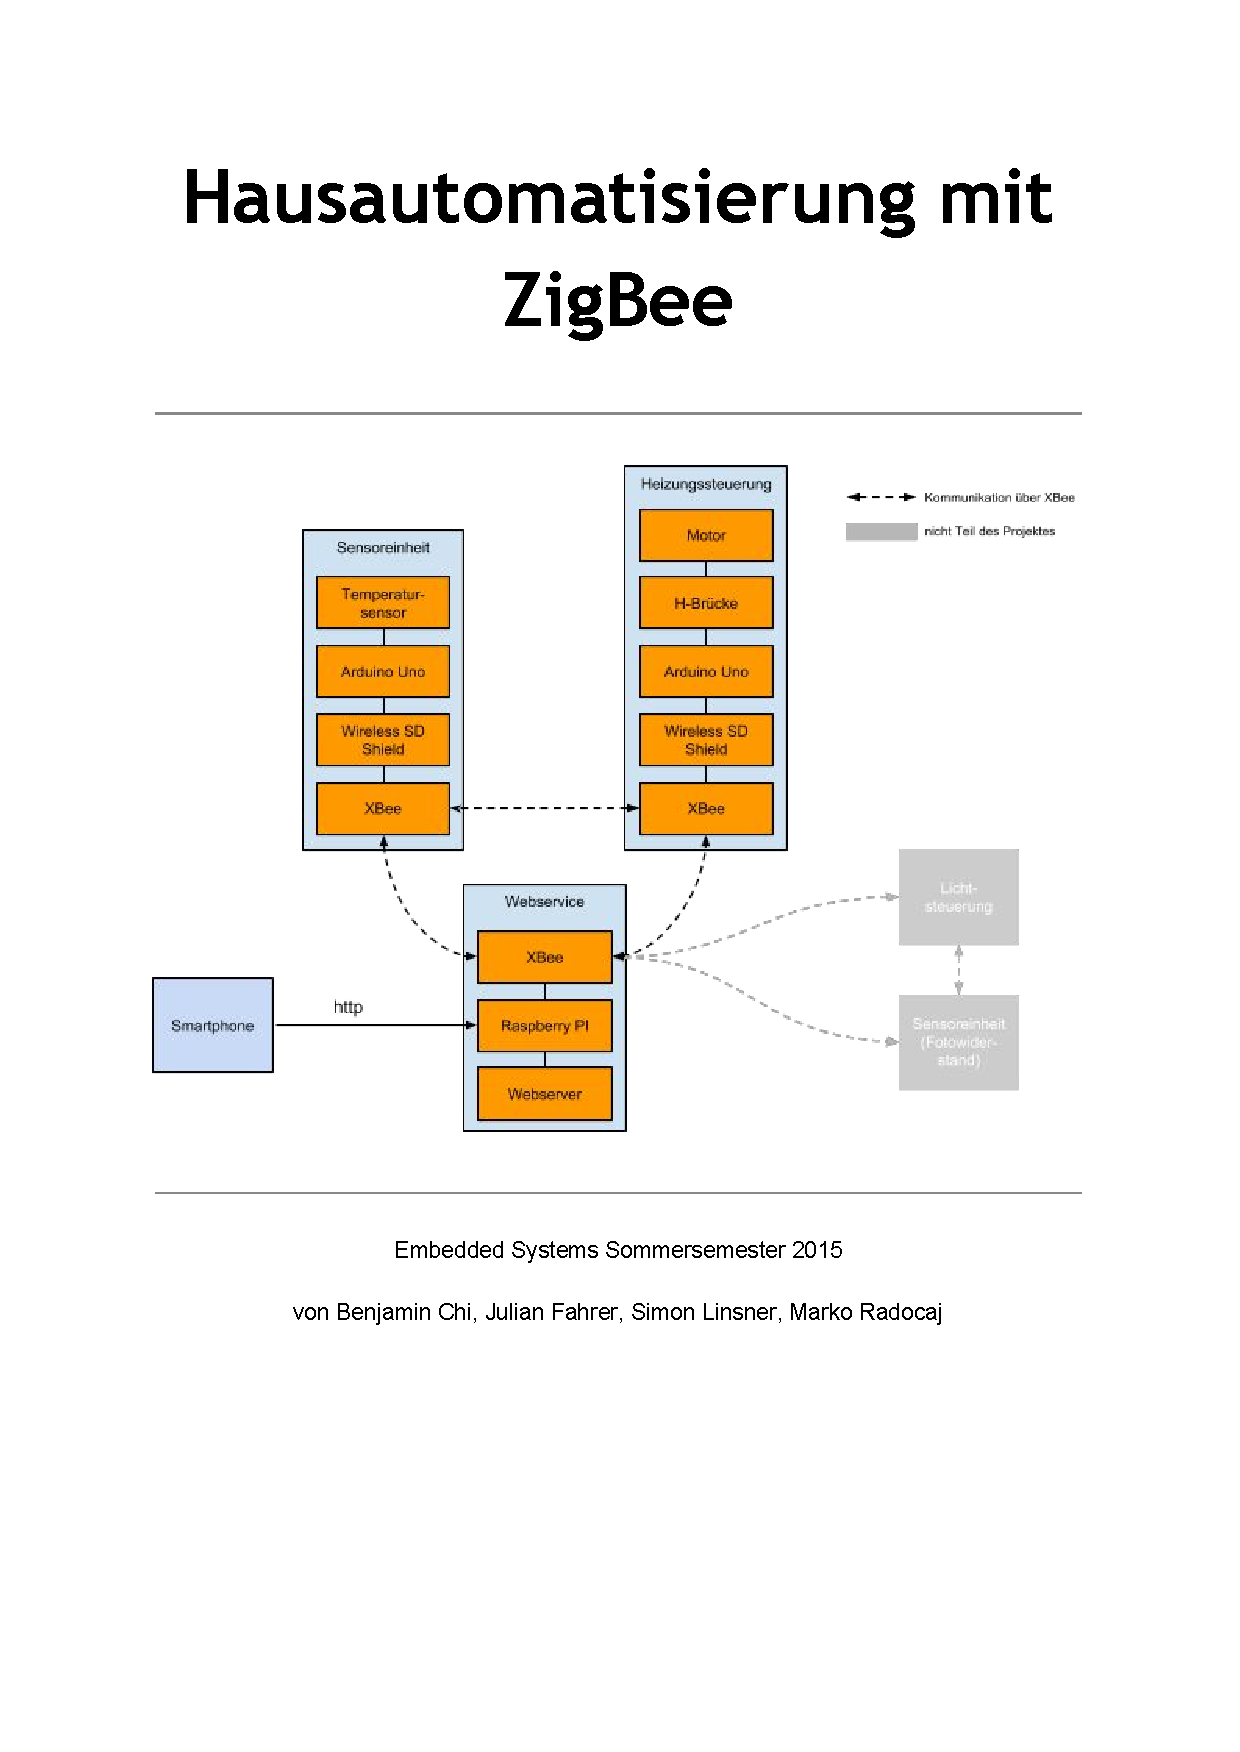
\includepdf[pagecommand={\thispagestyle{headings}},
%  pages=1-23, scale=0.8, frame=true]{Anhang/Dokumentation_SoSe2015.pdf}

